\setchapterstyle{kao}
\chapter{Experiments}
\labch{experiments}
This chapter outlines the experiments conducted to assess the efficacy of the
proposed loss formulation. To facilitate a comprehensive evaluation, multiple
neuroimaging datasets were utilized, which are described in a dedicated section.
Subsequent to dataset descriptions, the experimental setup is thoroughly
detailed, including the model used and all pertinent training parameters.
Finally, the chapter concludes with several sections, each dedicated to
discussing the experimental results for a specific task that was tested.

\section{Datasets}
Overall, the experimental data consisted of T1-weighted MRI scans, totaling
21,155 images from 7,908 individuals. This data was sourced from various
publicly available datasets, encompassing five different neurological
conditions. The conditions and respective datasets include healthy samples from
OpenBHB~\cite{dufumier_openbhb_2022}, Alzheimer's Disease from
ADNI~\cite{petersen_alzheimer_2010} and OASIS-3~\cite{lamontagne_oasis_2019},
schizophrenia from SchizConnect~\cite{wang_schizconnect_2016}, and Autism
Spectrum Disorder from ABIDE I~\cite{ABIDE}. This diverse compilation of
datasets provided a robust foundation for evaluating the proposed loss
formulation and its effectiveness across different neurological conditions.
The overall composition of the cohorts used in this study is presented in~\reftab{5_1}.
\begin{table}[h]
    \centering
    \caption[Cohorts Composition]{An overview of the various datasets utilized
    in this study, along with their cohort compositions.}
    \begin{tabular}{l l c}
    \toprule
    \textbf{Condition} & \textbf{Dataset} & \textbf{Patients}  \\
    \midrule
    Healthy Control & OpenBHB & 3984 \\
    Schizophrenia & SchizConnect & 383 \\
    Alzheimer's Disease & ADNI & 1754 \\
    Alzheimer's Disease & OASIS-3 & 685 \\
    Autism Spectrum Disorder & ABIDE-I & 1102 \\
    \bottomrule
    \end{tabular}
    \labtab{5_1}
\end{table}

\subsection{OpenBHB} OpenBHB is a newly released dataset that consolidates
healthy control (HC) samples from numerous public cohorts including ABIDE 1,
ABIDE 2, CoRR, GSP, IXI, Localizer, MPI-Leipzig, NAR, NPC, and RBP. Each scan in
this dataset originates from a different subject, making it uniquely suited for
ensuring diversity in the training process. In addition to structural scans and
patient information\sidenote{Some of them are age, sex, total intracranial
volume, acquisition settings.}, OpenBHB provides seven anatomical measures based
on the Desikan-Killiany parcellation~\cite{desikan_automated_2006}. As
previously discussed, such measures include cortical thickness (mean and
standard deviation), gray matter volume, surface area, integrated mean, Gaussian
curvature index, and intrinsic curvature index~\cite{dufumier_openbhb_2022}. 

\subsection{ADNI}
The Alzheimer's Disease Neuroimaging Initiative (ADNI) is a significant research
project that was launched to study Alzheimer's disease through the collection
and analysis of medical imaging, genetic, biological markers, and clinical
assessment data. ADNI is aimed at understanding the progression of Alzheimer's
Disease from its earliest stages, through mild cognitive impairment (MCI), to
full Alzheimer's Dementia (AD). Over the years, several phases of the
Alzheimer's Disease Neuroimaging Initiative (ADNI) have been undertaken, each
contributing to the growing body of data on Alzheimer's Disease and its
precursors. The specific phases include ADNI-1, ADNI-2, ADNI-GO, and ADNI-3. For
the experiments conducted, data from all these different ADNI phases were
utilized, comprising a diverse cohort of participants. This included 633 healthy
controls (HC), 712 patients diagnosed with mild cognitive impairment (MCI), and
409 patients diagnosed with Alzheimer's Disease (AD).

\subsection{OASIS-3}
The Open Access Series of Imaging Studies (OASIS-3) is a neuroimaging dataset
specifically designed for studying the progression of Alzheimer’s disease across
different stages. OASIS-3 builds upon earlier versions of the dataset (OASIS-1
and OASIS-2) by incorporating a larger and more diverse set of data points,
which includes both longitudinal and cross-sectional data. The dataset contains
a demographic of participants ranging from young adults to older adults with
varying stages of cognitive decline, including normal aging individuals, those
with Mild Cognitive Impairment (MCI), and those diagnosed with Alzheimer’s
disease. For the experiments conducted with this dataset, 685 patients were
included, containing 88 AD cases.

\subsection{SchizConnect}
SchizConnect is a dataset that emerged from a collaborative research effort
aimed at consolidating neuroimaging data from multiple studies and sites. It
includes participants diagnosed with schizophrenia, schizoaffective disorder,
other related psychotic disorders, and healthy control individuals. From the
SchizConnect database, anatomical MRIs were included for the experiments, for a
total of 383 patients. This cohort is categorized as follows: 180 are healthy
controls (HC), 102 are classified under schizophrenia (broad), 74 under
schizophrenia (strict), 11 as schizoaffective patients, and 9 with bipolar
disorder.

\subsection{ABIDE I}
The Autism Brain Imaging Data Exchange I (ABIDE-I) is an open-source initiative
designed to support research into Autism Spectrum Disorder (ASD). ABIDE-I
encompasses a comprehensive dataset comprising resting-state functional magnetic
resonance imaging (rs-fMRI) scans, anatomical scans, and phenotypic information
from over 1,000 individuals, ranging in age from 6 to 64 years. This diverse
group includes both individuals diagnosed with ASD and age-matched control
subjects without ASD, providing a robust resource for comparative studies.

In the conducted experiments, anatomical MRIs from ABIDE-I were utilized,
involving a total of 1,102 participants. This cohort was categorized into 556
healthy controls (HC), 339 patients diagnosed with autism, 93 patients with
Asperger's Syndrome, and 7 diagnosed with pervasive developmental disorder not
otherwise specified (PDD-NOS). 

\section{Experimental Settings}
\begin{figure*}
    \begin{subfigure}[t]{.45\linewidth}
        \caption{Pre-train phase}
        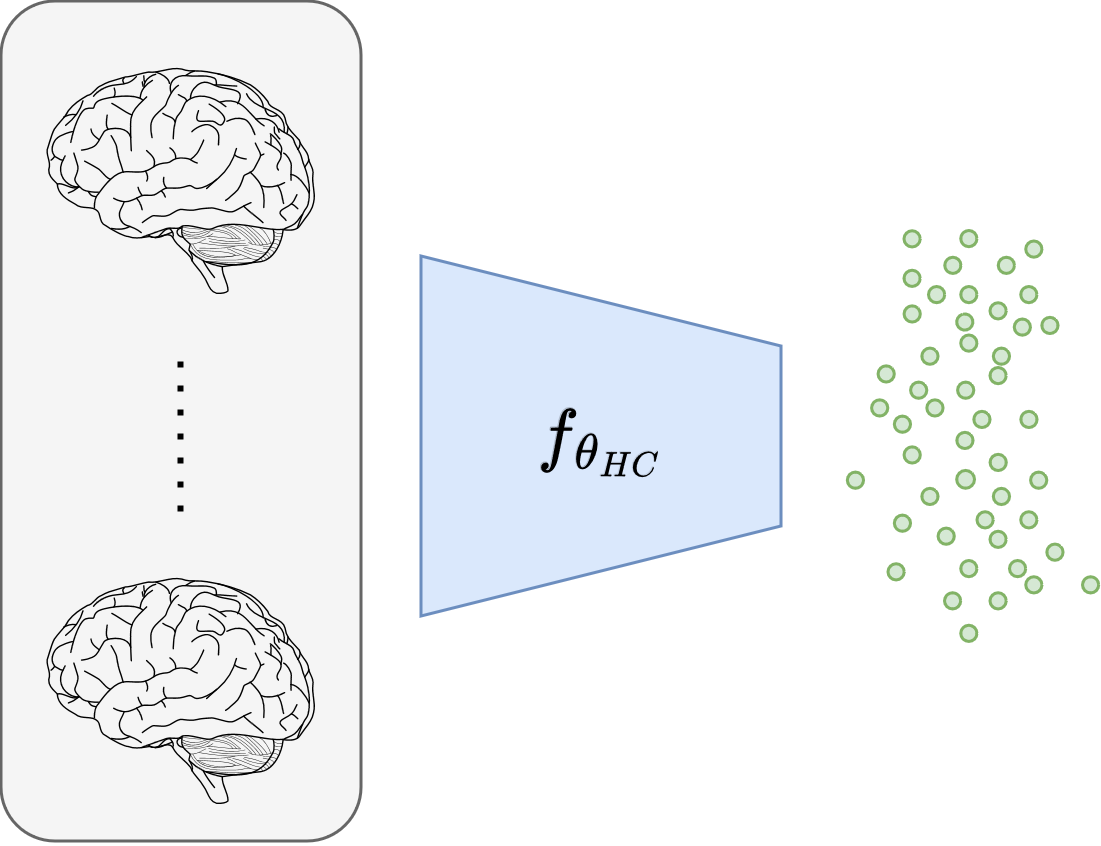
\includegraphics{5_1_a_pretrain}
    \end{subfigure}
    \hfill
    \begin{subfigure}[t]{.45\linewidth}
        \caption{Downstream transfer phase}
        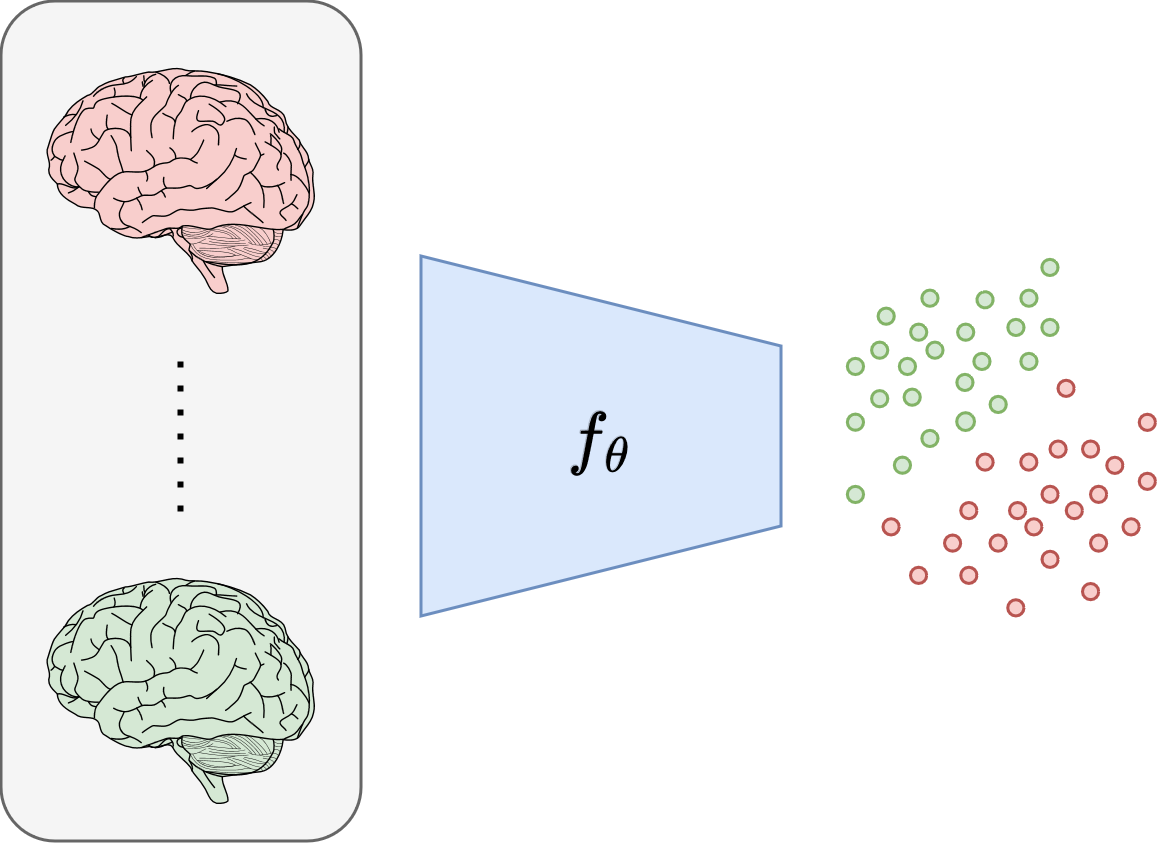
\includegraphics{5_1_b_transfer}
    \end{subfigure}
    \caption[Experimental Settings (Transfer Learning)]{
    The experimental settings adhere to the principles of transfer
    learning. Initially, a model $f$ (depicted in blue) is pre-trained on a
    substantial cohort of healthy subjects (represented by the grey box),
    utilizing the OpenBHB dataset in this instance. The outcome of this initial
    phase is a model $f_{\theta_{HC}}$, which has captured general variabilities
    within the data; that is, it has learned the latent \emph{manifold}. In the
    subsequent phase, the model is adapted to a downstream task. This involves
    mapping the images into the learned latent space, after which a conventional
    machine learning model is employed to perform the classification.
    }
    \labfig{}
\end{figure*}
Before initiating any experiments, to ensure uniformity across all images, they
underwent a standardized VBM preprocessing protocol using
CAT12~\cite{gaser_cat_2022}. This preprocessing included non-linear registration
to the MNI template and extraction of gray matter (GM). The images were brought
to a final spatial resolution of 1.5mm isotropic and sized to 121 x 145 x 121.
The preprocessing tasks were carried out using the BrainPrep
package~\sidecite{grigis_brainprep_2022}. The experiments specifically utilized
modulated gray matter (GM) images, as indicated by
~\citeauthor{dufumier_openbhb_2022}~\cite{dufumier_openbhb_2022}, to ensure that
the volumetric information was retained in the images for detailed analysis.

The experiments followed a two-phased approach aligned with the transfer
learning paradigm. Initially, a target model was pre-trained using the proposed
contrastive learning loss on the OpenBHB dataset. Subsequently, the model was
tested on various downstream tasks across different datasets to assess its
performance and generalization capabilities. Practically, in the proposed losses
(\refeqshort{4_7}, \refeqshort{4_8}), only a subset of the anatomical
measurements available in the Desikan format were utilized\sidenote{Specifically
Cortical Thickness (CT), Gray Matter Volume (GMV), and Surface Area (SA).}.
These losses are henceforth referred to as AnatCL-G3 for the global descriptor
version using three measurements and AnatCL-L3 for the corresponding local
descriptor.

The experimental settings for both loss formulations, local (AnatCL-L3) and
global (AnatCL-G3), were identical. Two ResNet-18 3D models were pre-trained
using VBM-preprocessed images along with their corresponding Desikan measures
based on the proposed formulations. The training process utilized the Adam
optimizer with a learning rate of 0.0001 and a decay rate of 0.9 applied every
10 epochs. The models were trained with a batch size of 32 for a total of 300
epochs. For simplicity, the values of $\lambda_1$ and $\lambda_2$ were both set
to 1. As is standard practice in contrastive learning approaches
~\cite{chen_self_contrastive_2020, khosla_supervised_contrastive_2021}, the
contrastive loss was computed using a fully-connected projection head following
the encoder, which consisted of two layers.

To endure a robust evaluation, the experimental setup included cross-validation,
where each of the 5 folds was structured with a 70\% training split and a 30\%
test split. This distribution ensured that each fold had a substantial amount of
data for training the models, while still providing a significant portion for
testing and evaluating model performance across different iterations. The
results were then quantified in terms of mean and standard deviation across the
5 folds, providing a comprehensive assessment of model performance and stability
across different test scenarios.

After the pre-training step, the models underwent evaluation by testing their
performance using a transfer learning approach. In this approach, latent
representations were first generated by the model using only the encoder
section, discarding the fully connected head\sidenote{This step ensures that the
evaluation focuses on the quality of the features extracted by the encoder,
rather than the classification capabilities of the full network.}. For each
downstream task, a different linear classifier was trained on these extracted
representations to assess the model's ability to learn meaningful and
generalizable features. The rationale behind this methodology was to isolate the
effectiveness of the learned representations from the specific architecture of
the downstream task classifiers. By focusing on the encoder's output, the
evaluation could better determine whether the fundamental features extracted
during pre-training were robust and informative enough to facilitate accurate
classifications across various conditions, independent of the subsequent
classifier configurations.

The downstream tasks primarily focused on predicting specific diagnoses (such as
Alzheimer's Disease, Schizophrenia, Bipolar Disorder, etc.), biomarkers (e.g.,
brain age), or phenotypes (e.g., sex). Additionally, other relevant clinical
assessments included in the datasets were also considered, which will be
explained in detail in~\refsec{cognitive_scores}. A total of 22 downstream tasks
were tested, which are summarized in~\reftab{5_2}.
\begin{table*}[h]
    \centering
    \caption[Downstream Tasks Summary]{Summary of downstream tasks (12) and
    clinical assessment scores (10) considered in the study.}
    \begin{tabular}{l l}
    \toprule
    \textbf{Dataset} & \textbf{Task / Condition} \\
    \midrule
    OpenBHB & Age (HC)   \\
            & Sex   \\
    ADNI    & Alzheimer's Disease \\
            & sMCI vs pMCI \\
    OASIS-3 & Alzheimer's Disease \\
    SchizConnect & Schizophrenia Broad \\
                 & Schizophrenia Strict \\
                 & Bipolar Disorder \\
                 & Schizoaffective \\
    ABIDE I & Autism \\
            & Aspergers \\
            & PDD-NOS \\
    \bottomrule
    \end{tabular}
    \begin{tabular}{l l}
    \toprule
    \textbf{Dataset} & \textbf{Phenotype}  \\
    \midrule
    SchizConnect  & AIMS Overall Severity  \\
                  & AIMS Upper Body \\
                  & AIMS Lower Body \\
                  & Depression \\
                  & Handedness \\
                  & SAS GAIT \\
    ABIDE 1 & Handedness \\
            & FIQ (WASI)\\
            & VIQ (WASI) \\
            & PIQ (WASI) \\
    & \\
    & \\
    \bottomrule
    \end{tabular}
    \labtab{5_2}
\end{table*}
For the comparative analysis with standard approaches, four different baseline
methodologies were also tested alongside the proposed method. These included the
completely self-supervised loss, known as SimCLR \sidenote{This loss was
introduced by the authors of the corresponding
paper~\cite{chen_self_contrastive_2020} and is referenced as such.}
(\refeqshort{4_2}), and three supervised baselines: a standard model trained
with the L1 loss \sidenote{An L1 loss function calculates the mean of the
absolute differences between the labels and the predictions.}, y-Aware
(\refeqshort{4_4}), and ExpW (\refeqshort{4_6}). To ensure consistency and
fairness in the evaluation, all these methods were subjected to the same
experimental setup as previously described. In this way, the comparative results
accurately reflect the relative performance of each method under identical
conditions.
All the experiments were implemented in PyTorch~\cite{paszke_2017} and run on a
cluster of 4 NVIDIA V100 GPUs\sidenote{The computational resources were provided
by the Leonardo supercomputer, which is managed by the CINECA consortium.}, with
each training session taking approximately 10 hours. 

\section{Diagnosis Prediction}
\begin{figure}
    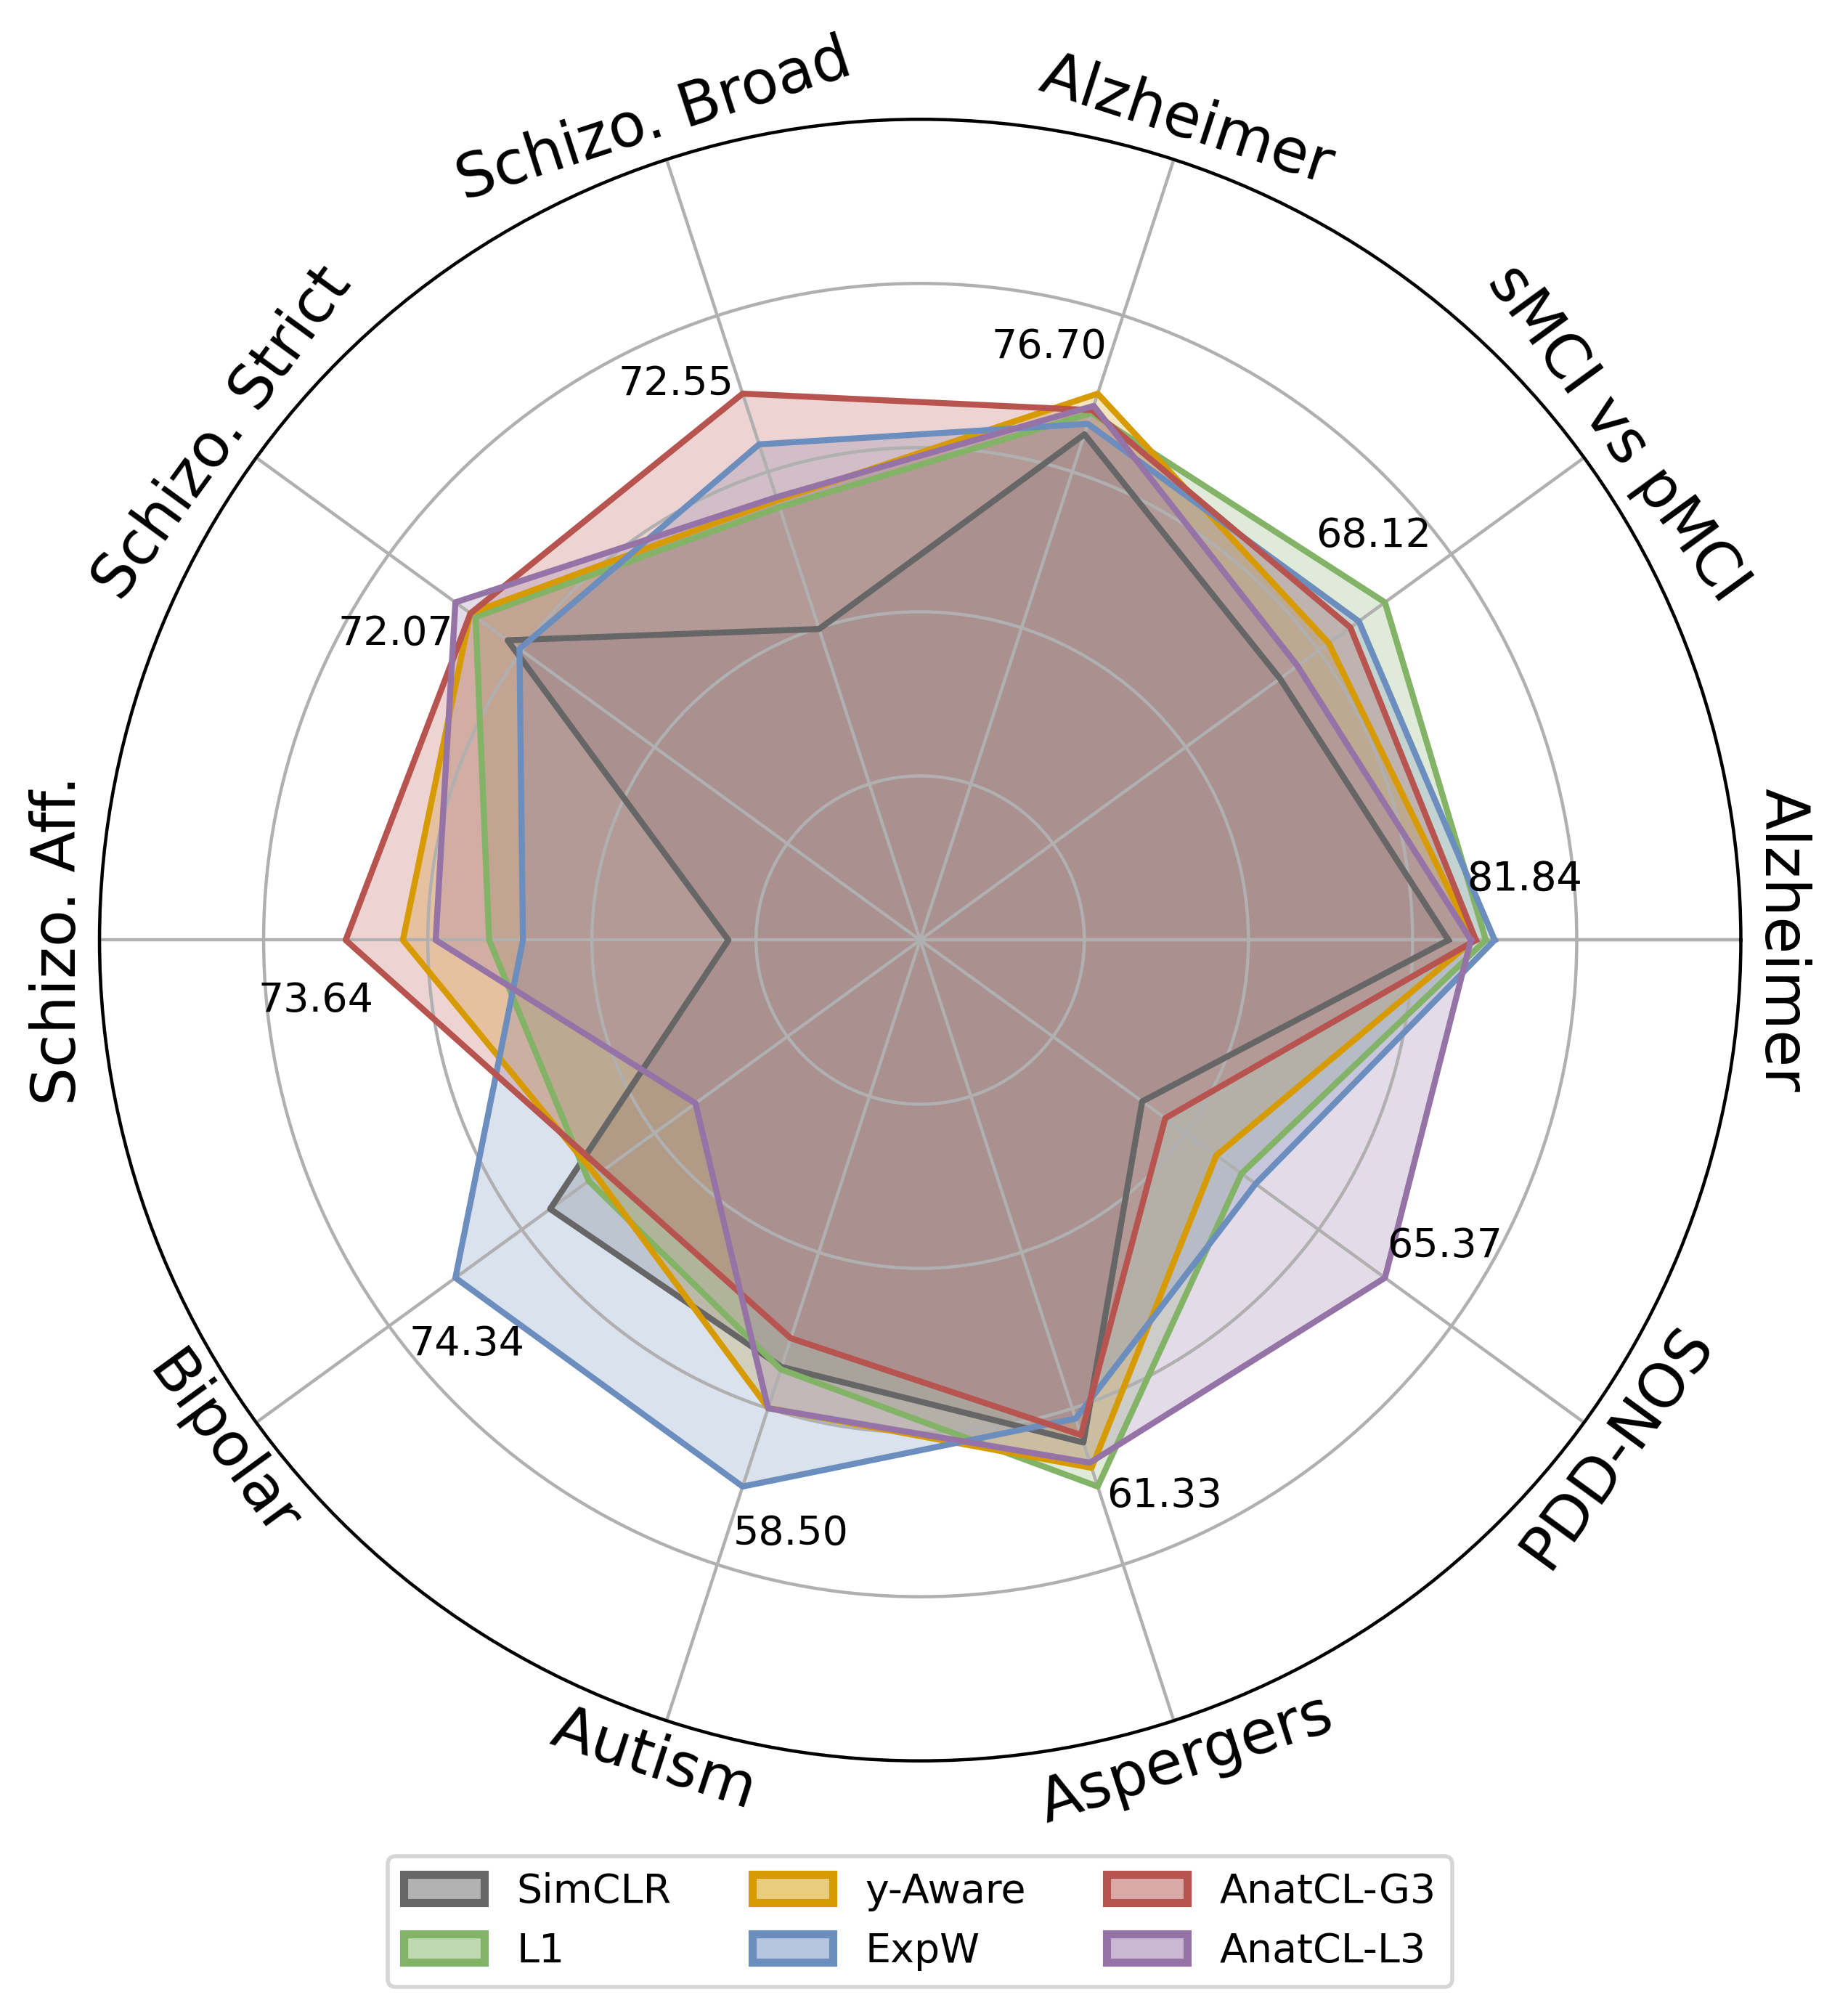
\includegraphics{5_2_polar_plot}
    \caption[Polar Plot of Various Tested Losses]{A polar plot that summarize
    the performances of the various loss functions discussed in this chapter.}
    \labfig{5_2}
\end{figure}

\subsection{Brain Age and Sex Prediction}
Preliminary results focusing on brain age prediction and sex classification were
evaluated using the OpenBHB dataset. These results are detailed
in~\reftab{5_3}. Analysis of the findings indicates that the
AnatCL model is capable of matching and slightly exceeding state-of-the-art
performance in brain age prediction tasks. It is important to note that no
bias-correction methods were employed in this study, despite recommendations
suggested by~\citeauthor{mayoral_biological_2023}~\cite{mayoral_biological_2023}
and ~\citeauthor{delange_commentary_2020}~\cite{delange_commentary_2020}. In
terms of sex classification, while the AnatCL model does not outperform the ExpW
approach, it does show improvements over the SimCLR and L1 loss baselines.
\begin{table}[!h]
    \centering
    \caption[Brain-Age Prediction Results]{Results on OpenBHB in terms of mean
    absolute error (MAE) on age prediction, and balanced accuracy on sex
    classification.}
    \begin{tabular}{l c c}
    \toprule
    \textbf{Method} & \textbf{Age MAE} & \textbf{Sex}  \\
    \midrule
    SimCLR & \result{5.58}{0.53} & \result{76.7}{1.67} \\
    %
    L1 (age sup.) & \result{2.73}{0.14} & \result{76.7}{0.67} \\
    %
    y-Aware & \result{2.66}{0.06} & \result{79.6}{1.13} \\
    %
    ExpW & \result{2.70}{0.06} & \textbf{\result{80.3}{1.7}} \\
    \midrule
    %
    AnatCL-G3 & \textbf{\result{2.61}{0.08}} & \result{78.2}{1.25} \\
    AnatCL-L3 & \result{2.64}{0.07} & \result{78.2}{0.7}\\
    \bottomrule
    \end{tabular}
    \labtab{5_3}
\end{table}

\subsection{Alzheimer's disease and Cognitive Impariments}
In~\reftab{5_4}, the results for Alzheimer's Disease (AD) detection using the
ADNI and OASIS-3 datasets are presented. Although the AnatCL model does not
achieve the best results overall, it generally shows improvements over the
self-supervised baseline (SimCLR) and occasionally surpasses the performance of
either the L1, y-Aware, or ExpW models. This indicates that while AnatCL may not
yet be the top-performing model across all metrics, it demonstrates potential by
consistently outperforming a self-supervised approach and, in some cases, other
supervised methodologies. This suggests that further refinement and adaptation
of the AnatCL approach could lead to more competitive results in AD detection
tasks, as will be discussed in \refch{conclusions_future_developments}.
\begin{table}[!h]
    \centering
    \caption[Alzheimer's Disease Results]{Results on Alzheimer's Disease (AD)
    classification in terms of balanced accuracy.}
    \begin{tabular}{l c c | c}
    \toprule
    & \multicolumn{2}{c|}{\textbf{ADNI}} & \multicolumn{1}{c}{\textbf{OASIS-3}}\\
    \textbf{Method} & \textbf{HC vs AD} & \textbf{sMCI vs pMCI} & \textbf{HC vs AD} \\
    \midrule
    SimCLR & \result{78.47}{2.51} & \result{61.77}{3.85} & \result{73.97}{4.98} \\
    L1 (age sup.) & \result{81.20}{2.3} & \textbf{\result{68.12}{5.42}} & \result{75.40}{5.4} \\
    y-Aware & \result{80.3}{1.8} & \result{64.72}{4.43} & \textbf{\result{76.70}{3.30}} \\
    ExpW & \textbf{\result{81.84}{2.95}} & \result{66.54}{5.64} & \result{74.67}{2.87} \\
    \midrule
    AnatCL-G3 & \result{80.47}{2.95} & \result{66.03}{2.93} & \result{75.59}{2.67}\\
    AnatCL-L3 & \result{80.11}{1.0} & \result{62.83}{4.5} & \result{75.88}{3.0}\\ 
    \bottomrule
    \end{tabular}
    %}
    \labtab{5_4}
\end{table}


\subsection{Schizophrenia and Bipolar Disorders}
The performance of downstream tasks on SchizConnect was evaluated for detecting
schizophrenia (broad and strict), schizoaffective, and bipolar disorders. The
results, detailed in~\reftab{5_5}, show that with the AnatCL model,
state-of-the-art performance was achieved in three out of the four tasks. This
underscores the value of incorporating anatomical information into the model,
particularly for these psychiatric conditions.

\begin{table*}[h]
    \caption[Schizophrenia Detection Results]{Results on schizophrenia detection
    (SCZ) in terms of balanced accuracy.}
    \begin{tabular}{l c c c c}
    \toprule
    &\multicolumn{4}{c}{\textbf{SchizConnect}}\\
    \textbf{Method} & \textbf{SCZ. (Broad)} & \textbf{SCZ (Strict)} & \textbf{Schizoaff.} & \textbf{Bipolar}\\
    \midrule
    SimCLR & \result{58.53}{3.52} & \result{68.47}{8.47} & \result{51.23}{11.94} & \result{67.34}{9.96}\\ 
    %
    L1 & \result{65.79}{4.74} & \result{70.68}{5.10} & \result{65.24}{15.21} & \result{64.49}{22.08} \\
    %
    y-Aware & \result{66.20}{4.50} & \result{71.04}{2.31} & \result{70.29}{14.73} & \result{63.95}{19.81} \\
    %
    ExpW & \result{69.53}{4.43} & \result{67.65}{8.27} & \result{63.26}{18.06} & \textbf{\result{74.34}{18.95}} \\
    %
    \midrule
    AnatCL-G3 & \textbf{\result{72.55}{5.16}} & \result{71.03}{8.53} & \textbf{\result{73.65}{7.29}} & \result{63.43}{15.94}\\
    %
    AnatCL-L3 & \result{66.38}{5.96} & \textbf{\result{72.07}{8.42}} & \result{68.37}{8.60} & \result{56.60}{11.48}\\
    \bottomrule
    \end{tabular}
    \hfill
    \labtab{5_5}
\end{table*}

\subsection{Autism Spectrum Disorder}
Additionally, the performance in detecting Autism Spectrum Disorder (ASD) across
three categories—autism, Asperger's, and PDD-NOS—is also reported
in~\reftab{5_6}. While AnatCL did not outperform other methods for autism and
Asperger's patients, it significantly improved accuracy for diagnosing patients
with PDD-NOS, a relatively rarer diagnosis within the dataset.
\begin{table}[h]
    \centering
    \caption[Autism Spectrum Disorder Detection Results]{Results on autism
    spectrum disorder (ASD) detection in terms of balanced accuracy.}
    \begin{tabular}{l c c c}
        \toprule
        &\multicolumn{3}{c}{\textbf{ABIDE-I}}\\
        \textbf{Method} & \textbf{Autism} & \textbf{Aspergers} & \textbf{PDD-NOS}\\
        \midrule
         SimCLR & \result{54.45}{2.99} & \result{59.61}{2.72} & \result{52.12}{6.62} \\
         L1 & \result{54.53}{1.79} & \textbf{\result{61.33}{8.77}} & \result{57.54}{5.93} \\
         y-Aware & \result{55.84}{3.37} & \result{60.60}{9.22} & \result{56.17}{10.17} \\
         ExpW & \textbf{\result{58.50}{2.41}} & \result{58.68}{3.82} & \result{58.31}{4.33} \\
         \midrule
         AnatCL-G3 & \result{53.48}{0.99} & \result{59.32}{6.58} & \result{53.38}{5.86} \\
         AnatCL-L3 & \result{55.85}{1.02} & \result{60.40}{2.29} & \textbf{\result{65.37}{6.73}} \\
         \bottomrule
    \end{tabular}
    \labtab{5_6}
\end{table}

Overall, AnatCL consistently outperformed or matched the other baselines,
demonstrating its efficacy across a diverse range of psychiatric conditions.
This suggests that AnatCL's approach to integrating detailed anatomical features
significantly contributes to its ability to detect nuanced differences in
neuroimaging data associated with various psychiatric diagnoses.

\section{Cognitive Scores/Assessments Prediction}
\labsec{cognitive_scores}
In the final experiments, the focus shifts to predicting clinical assessment
scores from brain MRIs, a topic that, to the best of current knowledge, has not
been extensively explored in other studies. Specifically, for the SchizConnect
dataset, evaluations included the Abnormal Involuntary Movement Scale (AIMS)
assessed across three domains (overall, upper body, lower body), a Depression
score based on the Calgary Scale, Handedness information, and GAIT measurements
with the Simpson-Angus-Scale (SAS). For the ABIDE dataset, assessments also
included handedness and three IQ scores\sidenote{IQ scores were measured using
the Wechsler Abbreviated Scale (WASI)}: Full Scale IQ (FIQ), Visual IQ (VIQ),
and Performance IQ (PIQ). 
\begin{figure*}[t]
    \begin{subfigure}[t]{.45\linewidth}
        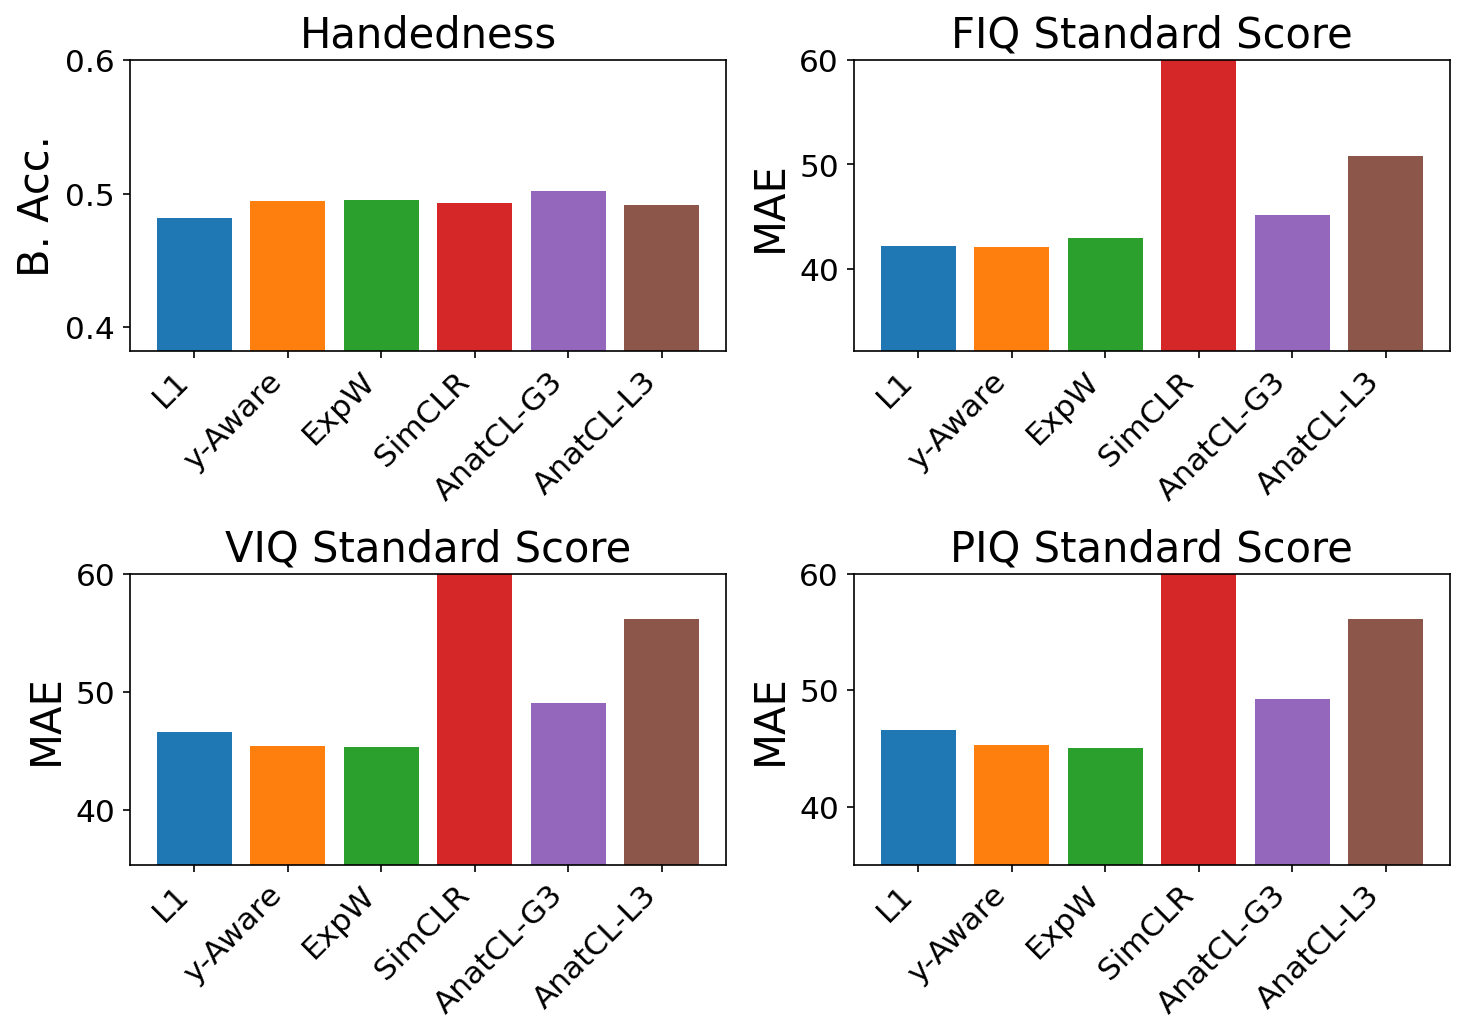
\includegraphics{5_3_a_abide_barplot}
        \caption{}
        \labfig{5_3_a}
    \end{subfigure}
    \hfill
    \begin{subfigure}[t]{.45\linewidth}
        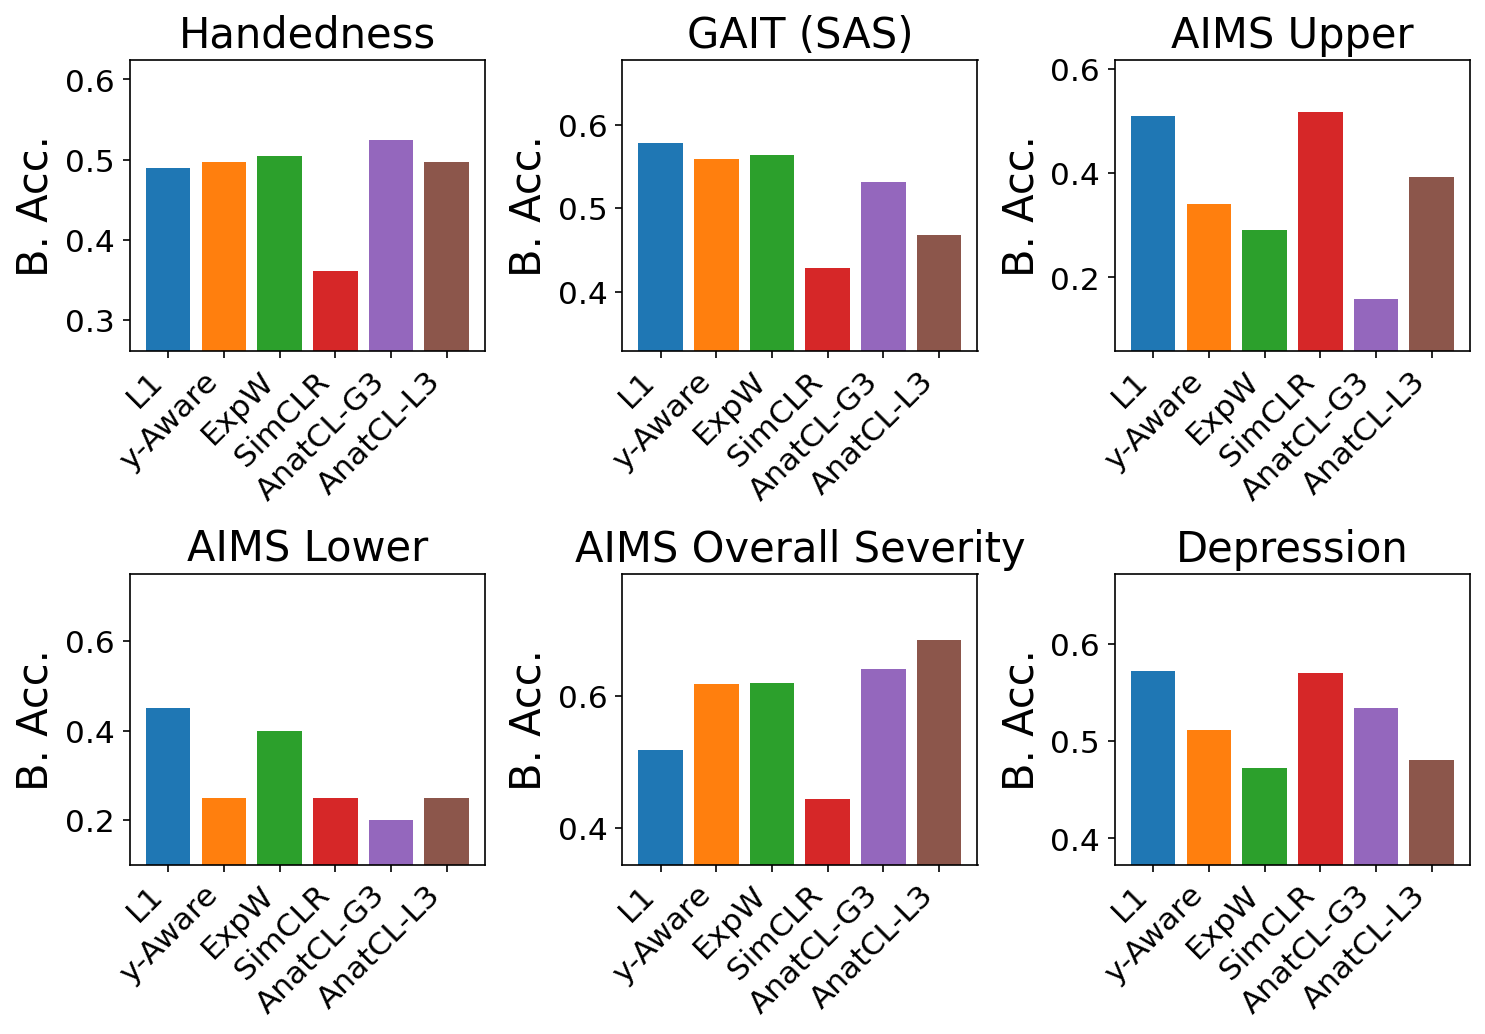
\includegraphics{5_3_b_schiz_barplot}
        \caption{}
        \labfig{5_3_b}
    \end{subfigure}
    \caption[Results Summary (Bar Plots)]{Bar plot format summarization of the
    results discussed. Subfigure~\ref{fig:5_3_a} refers to the ABIDE-I dataset,
    while subfigure~\ref{fig:5_3_b} on the SchizConnect.}
\end{figure*}

\begin{table*}[!b]
    \centering
    \caption[Assessment Scores Results on SchizConnect]{Results of assessment scores/phenotypes prediction from brain MRIs on the SchizConnect dataset.}
    \resizebox{\linewidth}{!}{%
    \begin{tabular}{l c c c c c c}
    \toprule
    & \multicolumn{6}{c}{\textbf{SchizConnect}}\\
     \textbf{Method} & \textbf{AIMS Overall} & \textbf{AIMS Up.} & \textbf{AIMS Low.} & \textbf{Depression} & \textbf{Handedness} & \textbf{GAIT} \\
    \midrule
    SimCLR & \result{44.33}{29.92} & \textbf{\result{51.67}{16.16}} & \result{25.00}{27.39} & \result{56.93}{13.88} & \result{36.06}{2.72} & \result{42.83}{9.61}\\
    %
    L1 & \result{51.83}{24.43} & \result{50.83}{20.82} & \textbf{\result{45.00}{33.17}} & \textbf{\result{57.17}{13.06}} & \result{48.91}{5.60} & \textbf{\result{57.73}{8.64}} \\
    %
    y-Aware & \result{61.83}{15.87} & \result{34.17}{11.90} & \result{25.00}{27.39} & \result{51.09}{5.32} & \result{49.71}{7.69} & \result{55.92}{9.52}\\
    %
    ExpW & \result{62.00}{12.40} & \result{29.17}{17.08} & \result{40.00}{33.91}
    & \result{47.26}{7.27} & \result{50.39}{6.28} &
    \result{56.39}{14.14}\\
    \midrule
    %
    AnatCL-G3 & \result{64.00}{12.72} & \result{15.83}{12.19} & \result{20.00}{18.71} & \result{53.35}{8.54} & \textbf{\result{52.44}{9.14}} & \result{53.10}{11.69} \\
    AnatCL-L3 & \textbf{\result{68.50}{18.09}} & \result{39.17}{14.81} &
    \result{25.00}{27.39} & \result{48.05}{10.89} & \result{49.67}{8.06} &
    \result{46.74}{5.05}\\
    \bottomrule
    \end{tabular}
    }
    \labtab{5_7}
\end{table*}

The ten phenotypes considered are divided based on the nature of the prediction
task: AIMS, depression, handedness, and GAIT are approached as classification
tasks, while IQ scores (FIQ, VIQ, and PIQ) are treated as regression tasks. More
precisely, for handedness, the model predicts right-handed versus other
(left-handed or ambidextrous); for depression, it classifies between absent
versus mild and above; for AIMS, it differentiates between none and minimal
versus mild and above; and for GAIT, it categorizes as normal versus everything
else The results of these experiments on the SchizConnect dataset are reported
in \reftab{5_7}, while the results regarding the ABIDE-I dataset
are reported in \reftab{5_8}.

\begin{table*}[!h]
    \caption[Assessment Scores Results on ABIDE-I]{Results of assessment scores/phenotypes prediction from brain MRIs on the ABIDE-I dataset.}
    \begin{tabular}{l c c c c}
    \toprule
    & \multicolumn{4}{c}{\textbf{ABIDE-I}} \\
    \textbf{Method} & \textbf{Handedness} & \textbf{FIQ (MAE)} & \textbf{VIQ (MAE)} & \textbf{PIQ (MAE)}\\
    \midrule
    SimCLR & \result{49.26}{5.78} & \result{84.65}{16.36} & \result{89.07}{15.14} & \result{89.68}{15.00}\\
    %
    L1 & \result{48.18}{9.43} & \result{42.16}{31.17} & \result{46.54}{32.57} & \result{46.64}{32.24}\\
    %
    y-Aware & \result{49.45}{1.56} & \textbf{\result{42.10}{31.14}} &
    \result{45.38}{33.19} & \result{45.35}{32.76} \\
    %
    ExpW  & \result{49.53}{3.26} & \result{42.94}{30.76} &
    \textbf{\result{45.28}{33.23}} & \textbf{\result{45.02}{32.88}} \\ 
    %
    AnatCL-G3 & \textbf{\result{50.21}{6.82}} & \result{45.18}{29.68} & \result{49.07}{31.52} & \result{49.30}{30.86} \\
    %
    AnatCL-L3 & \result{49.13}{3.32} & \result{50.77}{27.14} &
    \result{56.18}{28.06} & \result{56.13}{27.62}\\
    \bottomrule
    \end{tabular}
    \hfill
    \labtab{5_8}
\end{table*}

While it cannot be concluded that any of the analyzed methods can accurately
predict all clinical assessments from MRI scans, AnatCL overall achieves the
best results in three out of ten cases, which surpasses any other baseline
method. Interestingly, AnatCL shows a better capability to predict the overall
AIMS score and patients' handedness. This suggests that there may be a link
between brain anatomy and these specific phenotypes, highlighting the potential
of anatomically informed models in understanding and predicting behavioral
traits.

